\chapter{Black hole formation 2: Vaidya collapse}
\label{s:vai}

\minitoc

\section{Introduction}

Having investigated the gravitational collapse of a star, modeled as a ball of dust,
in the preceding chapter, we turn now to a less astrophysical scenario: the
formation of a black hole by the collapse of a spherical shell of pure radiation
(no matter!),
known as \emph{Vaidya collapse}. Albeit quite
academic, this process illustrates various features of black hole birth and dynamics,
in a way somehow complementary to the collapse of a dust ball.

\section{The ingoing Vaidya metric}

\subsection{General expression} \label{s:vai:general}

Let us consider a spherically symmetric spacetime $(\M,\w{g})$ described by
coordinates $(v,r,\th,\ph)$ such that $v\in \R$, $r\in(0, +\infty)$,
$\th\in(0,\pi)$ and $\ph\in(0,2\pi)$, $(\th,\ph)$ being standard
spherical coordinates on $\SS^2$ and $r$ being the areal radius associated
with spherical symmetry (cf. Sec.~\ref{s:sch:static_spher}).
The \defin{ingoing Vaidya metric}\index{ingoing!Vaidya metric}\index{Vaidya!metric!ingoing --}
is the metric tensor
\be \label{e:vai:Vaidya_metric_null}
    \encadre{ \w{g} =
            -\left( 1 - \frac{2 M(v)}{r} \right)\, \dd v^2
            + 2 \, \dd v \, \dd r
        + r^2 \left( \dd\th^2 + \sin^2\th\, \dd\ph^2 \right) } ,
\ee
where $M(v)$ is a real-valued function of $v$.
We immediately notice that this expression strongly resembles that
of the Schwarzschild metric expressed in the
\emph{null ingoing Eddington-Finkelstein}\index{Eddington-Finkelstein!coordinates}\index{null!ingoing Eddington-Finkelstein coordinates}
coordinates, as given by Eq.~(\ref{e:sch:Schwarz_metric_NIEF}). Actually, the
only difference is the constant $m$ in Eq.~(\ref{e:sch:Schwarz_metric_NIEF})
replaced by the function $M(v)$ in Eq.~(\ref{e:vai:Vaidya_metric_null}).
We may say that the Schwarzschild metric is the special case $M(v) = m$ of
the ingoing Vaidya metric.

A key property of the ingoing Vaidya metric is
\begin{greybox}
The hypersurfaces $v = \mathrm{const}$ are null; a normal to them is the (null)
vector\footnote{in index notation: $k^\alpha := - g^{\alpha\mu} \partial_\mu v = - \nabla^\alpha v \iff
k_\alpha := - \partial_\alpha v $.}:
\be \label{e:vai:def_k}
    \w{k} := - \vp{\dd v} = - \vw{\nabla} v \quad\iff\quad
    \uu{k} := - \dd v .
\ee
Moreover, $\w{k}$ is equal to minus the vector $\wpar_r$ of coordinates
$(v,r,\th,\ph)$:
\be \label{e:vai:k_d_dr}
    \w{k} = - \left. \der{}{r} \right| _{v,\th,\ph} ,
\ee
where we have rewritten $\wpar_r$ as $\left. \dert{}{r} \right| _{v,\th,\ph}$
to distinguish it from the vector $\wpar_r$ of the IEF coordinates, to be
introduced in Sec.~\ref{s:vai:IEF}.
\end{greybox}
\begin{proof}
Let $\Sigma_v$ be a hypersurface defined by $v = \mathrm{const}$.
The metric induced by $\w{g}$ on $\Sigma_v$
is obtained by setting $\dd v = 0$ in Eq.~(\ref{e:vai:Vaidya_metric_null}):
$\left.\w{g}\right| _{\Sigma_v} = r^2 \left( \dd\th^2 + \sin^2\th\, \dd\ph^2 \right)$.
This metric has clearly the signature $(0, +, +)$, i.e. it is degenerate, hence
$\Sigma_v$ is a null hypersurface (cf. Sec.~\ref{s:def:hor_as_null}).
By construction, $\w{k}$ is normal to $\Sigma_v$. It is thus a null vector.
Besides, the metric dual of
the coordinate vector field $\wpar_r$ is the 1-form
$\uu{\wpar_r} = g_{\mu r}\dd x^\mu = g_{vr} \dd v = \dd v = - \uu{k}$,
which proves Eq.~(\ref{e:vai:k_d_dr}).
\end{proof}

Since $\dd v$ is nowhere vanishing, $\w{k}$ is a nonzero null vector field on $\M$.
We may use it to set up the \emph{time orientation} of $(\M,\w{g})$
by declaring that $\w{k}$ is future-oriented (cf. Sec.~\ref{s:fra:time_orientation}).

As shown in the notebook~\ref{s:sam:Vaidya},
the Ricci tensor of $\w{g}$ takes a simple form:
\be \label{e:vai:Ricci_tensor}
    \w{R} = \frac{2 M'(v)}{r^2}\, \dd v \otimes \dd v ,
\ee
where $M'(v)$ stands for the derivative of the function $M(v)$.
The Ricci scalar $R = g^{\mu\nu} R_{\mu\nu} = (2M'(v)/r^2) \, \nabla_\mu v \nabla^\mu v =  (2M'(v)/r^2) \, k_\mu k^\mu$ is identically zero, since $\w{k}$ is a null vector.
It follows that
\begin{greybox}
The ingoing Vaidya metric (\ref{e:vai:Vaidya_metric_null}) is a solution
of the Einstein equation (\ref{e:fra:Einstein_eq})
with $\Lambda = 0$ and with the energy-momentum tensor
\be \label{e:vai:ener_mom_tensor}
   \encadre{ \w{T} = \frac{M'(v)}{4\pi r^2}\, \uu{k} \otimes \uu{k}  } .
\ee
\end{greybox}

\begin{remark}
We have already noticed that Vaidya metric reduces to Schwarzschild metric for $M(v) = \mathrm{const}$.
This corresponds to $M'(v) = 0$, so that
Equation~(\ref{e:vai:ener_mom_tensor}) reduces to $\w{T} = 0$ and we recover that
Schwarzschild metric is a solution of the vacuum Einstein equation.
\end{remark}

The tensor (\ref{e:vai:ener_mom_tensor}) has the same
structure as the energy-momentum tensor of the dust model considered in Chap.~\ref{s:lem}:
$\w{T}_{\rm dust} = \rho  \, \uu{u} \otimes \uu{u} $ [Eq.~(\ref{e:lem:T_pressureless})].
The main difference is that $\w{u}$ is a timelike vector (the dust 4-velocity), while
$\w{k}$ is a null vector. For this reason, the energy-momentum tensor  (\ref{e:vai:ener_mom_tensor})
is sometimes referred to as a \defin{null dust}\index{null!dust}\index{dust!null --} model \cite{Poiss04}.
It corresponds physically to the energy-momentum tensor of some \emph{monochromatic electromagnetic radiation} in the
\emph{geometrical optics}\index{geometrical optics} approximation (see Box~22.4 of Ref.~\cite{MisneTW73}):
$\w{T}_{\rm rad} = q  \, \uu{K} \otimes \uu{K}$, where $q\geq 0$ and $\w{K} := \vw{\nabla}\Phi$ is the \emph{wave vector}\index{wave!vector}, $\Phi$ being the rapidly-varying
phase in the geometrical optics decomposition $\w{A} = \mathrm{Re}(\mathrm{e}^{\mathrm{i}\Phi} \, \w{a})$ of the electromagnetic potential 1-form $\w{A}$. The quantity $q$ is related to the energy density
$\veps$ of the electromagnetic field as measured by an observer $\Obs$ of 4-velocity $\w{u}$
by $\veps = \omega^2 q$, where $\omega = - \w{K}\cdot\w{u}$ is the frequency of the electromagnetic
radiation as measured by $\Obs$.
Maxwell equations\index{Maxwell equations} imply that $\w{K}$ is a null vector and that it is geodesic:
$\w{\nabla}_{\w{K}}\, \w{K} = 0$. The geodesic integral curves of $\w{K}$ are nothing but
the \emph{light rays}\index{light!ray} of the geometrical optics framework.
The geodesic character also holds for $\w{k}$ as defined by Eq.~(\ref{e:vai:def_k}),
since $\w{k}$ is normal to the null hypersurfaces $v = \mathrm{const}$:
the integral curves of $\w{k}$ are the null geodesic generators of these hypersurfaces
(cf. Sec.~\ref{s:def:null_geod_gen}); moreover,
we have exactly
\be \label{e:vai:k_geodesic}
    \w{\nabla}_{\w{k}}\, \w{k} = 0 .
\ee
This follows from Eq.~(\ref{e:def:wl_geod_kappa}) with $\wl = \w{k}$ and $\kappa = 0$
by virtue of Eq.~(\ref{e:def:def_kappa}) with $\rho=0$ implied by
Eq.~(\ref{e:def:wl_rho_u}) given that $u = v$ and $\w{k} =  - \vw{\nabla} v$ [Eq.~(\ref{e:vai:def_k})].
Equations~(\ref{e:vai:k_geodesic}) and (\ref{e:vai:k_d_dr})
imply that the curves $(v,\th,\ph) = \mathrm{const}$
are null geodesics, $\lambda:=-r$ is an affine parameter along them and $\w{k}$ is
the corresponding tangent vector.

Another condition for the identification of $\w{T}$ with $\w{T}_{\rm rad}$ is that the coefficient
in front of $\uu{k} \otimes \uu{k}$ in (\ref{e:vai:ener_mom_tensor})
is non-negative, since $q\geq 0$ in $\w{T}_{\rm rad}$. This constraint can also be seen as the \emph{null energy condition} (\ref{e:neh:null_energy_cond}) introduced in
Sec.~\ref{s:neh:NEH_Theta_zero}: for any null vector $\wl$, we have
$\w{T}(\wl,\wl) = M'(v)/(4\pi r^2)\, (\w{k}\cdot\wl)^2$ and hence $\w{T}(\wl,\wl) \geq 0$ $\iff$
$M'(v) \geq 0$. In other words, the function $M(v)$ must be monotically increasing. Then, we can set
$\w{k} = \alpha \w{K}$, where $\alpha$ is a constant, to have a perfect match of (\ref{e:vai:ener_mom_tensor}) with the electromagnetic radiation energy-momentum
tensor $\w{T}_{\rm rad}$.
To summarize:
\begin{greybox}
Provided that $M(v)$ is an increasing function\footnote{by \emph{increasing}, it is meant
strictly increasing ($M'(v)>0$) or locally constant ($M'(v) = 0$).},
the ingoing Vaidya spacetime $(\M,\w{g})$ is generated by a spherical symmetric electromagnetic radiation
within the geometrical optics approximation. The corresponding light rays are the
\defin{ingoing radial null geodesics}\index{ingoing!radial!null geodesics}
defined by $v=\mathrm{const}$, $\th=\mathrm{const}$ and $\ph=\mathrm{const}$.
These geodesics admit $\w{k}$ as the tangent vector associated with their affine parameter
$\lambda := -r$.
\end{greybox}

\subsection{Expression in ingoing Eddington-Finkelstein coordinates} \label{s:vai:IEF}

To deal with the black hole formation in Vaidya spacetime, it is quite
convenient to work with the
\defin{ingoing Eddington-Finkelstein (IEF) coordinates}\index{Eddington-Finkelstein!coordinates}\index{ingoing!Eddington-Finkelstein!coordinates}\index{IEF}
$(t,r,\th,\ph)$ defined from the null coordinates $(v,r,\th,\ph)$ in the
same way as for the Schwarzschild case, i.e. such that $v$ is the
\defin{advanced time}\index{advanced!time}\index{time!advanced --} with respect to $t$
[cf. Eq.~(\ref{e:sch:ti_v_r})]:
\be  \label{e:vai:t_v_r}
    \encadre{t := v - r} \iff \encadre{v = t + r} .
\ee
\begin{remark}
The coordinate $t$ was denoted by $\ti$ in Chap.~\ref{s:sch}, where $t$
was reserved for the Schwarzschild-Droste time coordinate.
\end{remark}
We have $\dd v = \dd t + \dd r$, from which the IEF expression of the
metric tensor is immediately deduced from Eq.~(\ref{e:vai:Vaidya_metric_null}):
\be \label{e:vai:metric_IEF}
    \encadre{
        \begin{array}{ll}
        \w{g} = &
           \displaystyle -\left( 1 - \frac{2 M(t+ r)}{r} \right)\, \dd t^2
            + \frac{4 M(t + r)}{r} \, \dd t \, \dd r
            + \left( 1 + \frac{2 M(t+r)}{r} \right)\, \dd r^2 \\[1ex]
       & + r^2 \left( \dd\th^2 + \sin^2\th\, \dd\ph^2 \right) .
       \end{array}
       }
\ee
The expression of $\w{k}$ in terms of the IEF coordinate frame
is deduced from Eq.~(\ref{e:vai:k_d_dr}) and the chain rule:
\be \label{e:vai:k_IEF}
    \w{k} = \wpar_t - \wpar_r .
\ee
\begin{remark}
The analog equation in Schwarzschild spacetime is Eq.~(\ref{e:sch:null_vector_k}).
\end{remark}

\subsection{Outgoing radial null geodesics}

Let us determine the radial null directions at each point by searching for
null vectors of the form $\wl = \wpar_t + V \wpar_r$. The condition
$\w{g}(\wl, \wl) = 0$ with the expression (\ref{e:vai:metric_IEF}) for
$\w{g}$ yields immediately a quadratic equation for $V$:
\[
    \left( 1 + \frac{2 M(t+r)}{r} \right) V^2
    + \frac{4 M(t + r)}{r}\, V +
    1 - \frac{2 M(t+ r)}{r}  = 0 .
\]
The two solutions are $V = -1$ and $V = [r - 2M(t + r)]/[r + 2M(t+r)]$.
The first solution gives back the ingoing null vector $\w{k}$ introduced in Sec.~\ref{s:vai:general}
[cf. Eq.~(\ref{e:vai:k_IEF})].
The null vector $\wl$ corresponding to the second solution is
\be
    \wl = \wpar_t + \frac{r - 2M(t + r)}{r + 2M(t+r)}\, \wpar_r .
\ee

\begin{greybox}
The integral curves of the vector fields $\w{k}$ and $\wl$ are null geodesics.
Those of $\w{k}$ are the \emph{ingoing radial null geodesics}\index{ingoing!radial!null geodesic}
already discussed in Sec.~\ref{s:vai:general},
while those of $\wl$ are called the \defin{outgoing radial null geodesics}\index{ingoing!null geodesic}.
\end{greybox}

\begin{proof}
A direct computation shows that $\wl$ is a pregeodesic vector field:
$\wnab_{\wl} \wl = \kappa \wl$, with $\kappa = - 4 [rM'(t+r) - M(t+r)]/[r + 2M(t+r)]^2$
(cf. the notebook~\ref{s:sam:Vaidya}). It follows that the integral curves of
$\wl$ are geodesics (cf. Sec.~\ref{s:geo:gener_param}).
\end{proof}
The differential equation governing the outgoing radial null geodesics
is obtained by demanding that $\wl$ is their tangent vector:
\be \label{e:vai:ODE_outgoing_null}
    \frac{\D r}{\D t} = \frac{r - 2M(t + r)}{r + 2M(t+r)} .
\ee

\begin{remark}
As in the Schwarzschild case (cf. Remark~\ref{r:sch:outgoing_ingoing}
on p.~\pageref{r:sch:outgoing_ingoing}),
the outgoing radial null geodesics are actually \emph{ingoing}, i.e. have $r$ decreasing towards the future,
as soon as $r < 2 M(t+r)$. This corresponds to the region bounded by the red curve in Fig.~\ref{f:vai:diag_S0}.
\end{remark}

%%%%%%%%%%%%%%%%%%%%%%%%%%%%%%%%%%%%%%%%%%%%%%%%%%%%%%%%%%%%%%%%%%%%%%%%%%%%%%%

\section{Infalling shell of radiation}

\subsection{The infalling shell model}

An \defin{infalling shell of radiation}\index{shell!infalling -- of radiation}\index{infalling!shell of radiation}
is defined by the ingoing Vadya metric with the function $M(v)$ obeying
$M'(v) \neq 0$ only on a finite interval of $v$. By choosing properly
the origin of $v$, we may consider this interval to be $[0, v_0]$, with
the parameter $v_0>0$ governing the
thickness of the shell.
The function $M(v)$ is thus constant outside the interval $[0, v_0]$.
In order to describe the formation of a black hole, we choose
$M(v) = 0$ for $v < 0$. This corresponds to a piece of Minkowski spacetime,
since the metric (\ref{e:vai:metric_IEF})
cleary reduces to Minkowski metric wherever $M(v)=0$ [compare Eq.~(\ref{e:glo:Mink_metric_spher})].
Denoting by $m>0$ the constant value of $M(v)$ for $v > v_0$, we have then
\be \label{e:vai:mass_function}
    M(v) = \left\{ \begin{array}{ll}
     0 \quad \mbox{for} \ v < 0 \qquad & \mbox{(Minkowski region)} \\
     m \, S(v/v_0) \quad \mbox{for} \ 0 \leq v \leq v_0
        & \mbox{(radiation region)} \\
      m \quad \mbox{for} \ v > v_0 \qquad & \mbox{(Schwarzschild region),}
      \end{array} \right.
\ee
where $S: [0,1] \to [0,1],\ x \mapsto S(x)$ is an increasing function
obeying $S(0) = 0$ and $S(1) = 1$.
The region for $v>v_0$ is qualified as \emph{Schwarzschild} since for $M(v) = m = \mathrm{const}$,
the Vaidya metric reduces to Schwarzschild metric, as noticed
in Sec.~\ref{s:vai:general}.
The three regions are shown in terms of coordinates $(t, r)$ on Fig.~\ref{f:vai:diag_S0}:
the radiation region (the infalling shell) is painted in yellow, the Minkowski
region lies below it and the Schwarzschild region lies above it.

\begin{figure}
\centerline{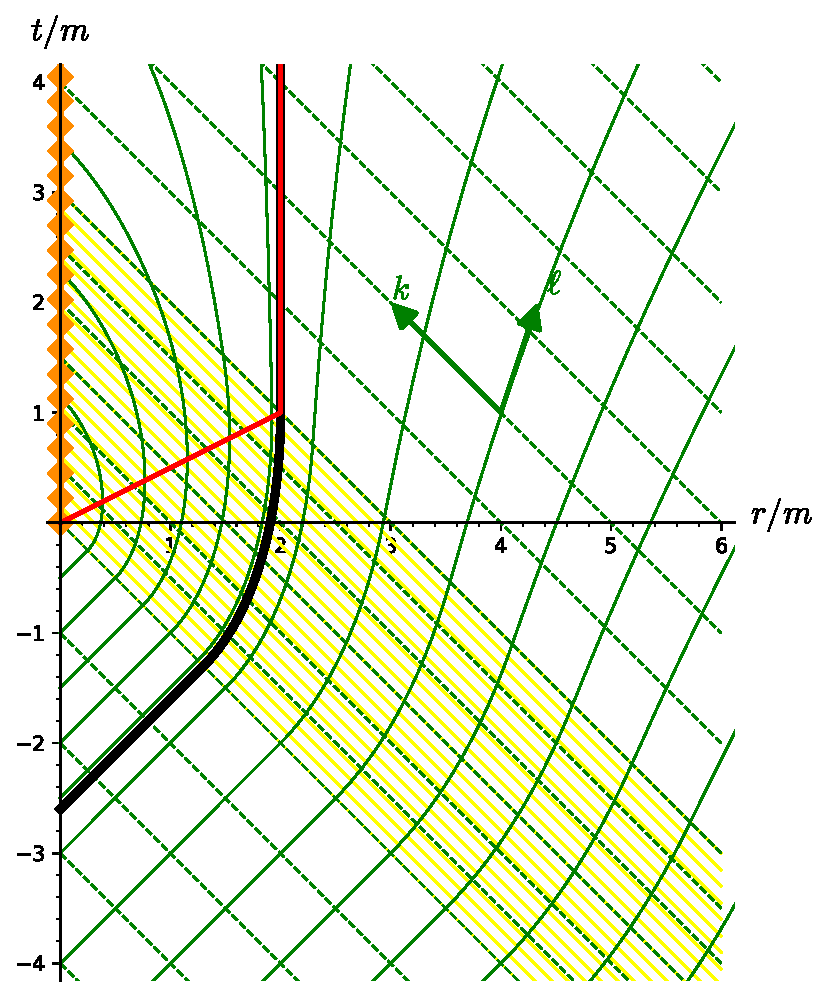
\includegraphics[width=0.6\textwidth]{vai_diag_S0.pdf}}
\caption[]{\label{f:vai:diag_S0} \footnotesize
Spacetime diagram of the Vaidya collapse based on the IEF coordinates $(t, r)$
and for the linear mass function $M(v)=m v/v_0$ with $v_0 = 3 m$.
The yellow area is the radiation region [cf. Eq.~(\ref{e:vai:mass_function})],
below it lies the Minkowski region and above it the Schwarzchild one.
The solid (resp. dashed) green curves are outgoing (resp. ingoing) radial
null geodesics. The thick black line marks the event horizon and
the red one the future outer trapping horizon. The curvature singularity
is indicated by the orange zigzag line. The part of the figure corresponding
to the Minkowski region can be compared with Fig.~\ref{f:glo:null_coord},
while that corresponding to the Schwarzschild region can be
compared with Fig.~\ref{f:sch:rad_null_geod_EF}.
\textsl{[Figure generated by the notebook \ref{s:sam:Vaidya}]}
}
\end{figure}


The simplest example of a function $M(v)$
obeying (\ref{e:vai:mass_function}) is obtained for $S(x) = x$:
\be \label{e:vai:S_linear}
     S(x) = x \quad \iff \quad M(v) = m \frac{v}{v_0} \quad (0 \leq v \leq v_0).
\ee
It is shown as the blue curve in Fig.~\ref{f:vai:mass_function}.
This choice of $S$ makes $M(v)$ piecewise linear. The resulting metric tensor
(\ref{e:vai:Vaidya_metric_null}) is continuous but not $C^1$ at $v=0$ and $v=v_0$. A choice
of $S$ that yields a $C^2$ metric tensor is
\be
    S(x) = 6 x^5 - 15 x^4 + 10 x^3 .
\ee
This choice is depicted by the red curve in Fig.~\ref{f:vai:mass_function}.

\begin{figure}
\centerline{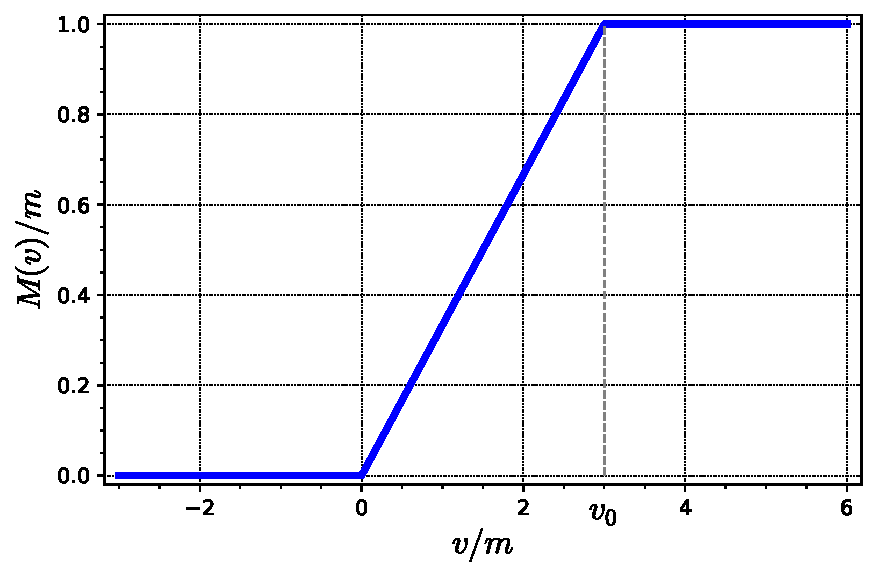
\includegraphics[width=0.6\textwidth]{vai_mass_function.pdf}}
\caption[]{\label{f:vai:mass_function} \footnotesize
Function $M(v)$ for the infalling shell model, for $v_0 = 3 m$ and
two different choices of $S(x)$ in formula~(\ref{e:vai:mass_function}).
}
\end{figure}

\subsection{Solution for $M(v)$ piecewise linear} \label{s:vai:sol_M_linear}

Let us consider the simplest choice for $M(v)$, i.e.
Eq.~(\ref{e:vai:S_linear}).
In the radiation region, the metric tensor (\ref{e:vai:Vaidya_metric_null})
takes the form
\be \label{e:vai:self_similar_metric}
    \w{g} = -\left( 1 - \alpha \frac{v}{r} \right)\, \dd v^2
            + 2 \, \dd v \, \dd r
        + r^2 \left( \dd\th^2 + \sin^2\th\, \dd\ph^2 \right) \qquad
        (0 \leq v \leq v_0),
\ee
where $\alpha$ is the positive constant defined by
\be \label{e:vai:def_alpha}
   \encadre{ \alpha := \frac{2m}{v_0} }.
\ee
It is immediately apparent on (\ref{e:vai:self_similar_metric})
that for any $\lambda > 0$, the homothety $H_\lambda:\ (v, r) \mapsto (\lambda v, \lambda r)$
maps $\w{g}$ to $\lambda^2 \w{g}$. Hence $H_\lambda$ is a
conformal isometry\index{conformal!isometry}\index{isometry!conformal --} of
$\w{g}$ with a constant conformal factor $\lambda^2$. The homotheties $(H_\lambda)_{\lambda\in \R_{>0}}$
form a 1-dimensional
group, the generator of which is obtained by considering infinitesimal transformations,
i.e. homotheties of ratio $\lambda = 1 + \D\lambda$ where $\D\lambda$ is
infinitely small. The components of the corresponding displacement vector are $\D v = \D\lambda \, v$
and $\D r = \D\lambda\,  r$, so that formula~(\ref{e:neh:xi_dxdt}) (with $t \leftrightarrow \lambda$)
leads to the generator
\be
    \w{\xi} = v \, \wpar_v + r \left. \wpar_r \right| _{v,\th,\ph}
            = t \, \wpar_t + r \, \wpar_r .
\ee
The second equality follows form the change of coordinates (\ref{e:vai:t_v_r}).
That $\w{\xi}$ has the same expression with respect to $(v, r)$ and $(t, r)$
coordinates should not be surprising since the homothety $H_\lambda$ has the
same expression in both coordinate systems:  $H_\lambda:\ (t, r) \mapsto (\lambda t, \lambda r)$,
given that $\lambda v = \lambda(t + r) = \lambda t + \lambda r$.
The vector field $\w{\xi}$ is called a
\defin{homothetic Killing vector}\index{homothetic!Killing vector}\index{Killing!vector!homothetic --}.
The Lie derivative of $\w{g}$ along $\w{\xi}$ is twice $\w{g}$ (cf. the notebook~\ref{s:sam:Vaidya}
for the computation):
\be \label{e:vai:Lie_xi_g}
    \Lie{\xi} \w{g} = 2 \w{g} .
\ee

\begin{remark}
A \emph{homothetic Killing vector} is not a \emph{Killing vector},
for the right-hand side of Eq.~(\ref{e:vai:Lie_xi_g}) would be zero if
$\w{\xi}$ were a Killing vector [cf. Eq.~(\ref{e:neh:Lie_xi_g})].
In other words, except for $\lambda=1$, the homotheties $H_\lambda$ are not isometries,
but only conformal isometries.
Generally, vector fields generating conformal isometries are
called \defin{conformal Killing vectors}\index{conformal!Killing vector}.
They fulfill $\Lie{\xi} \w{g} = \sigma \w{g}$, where $\sigma$ is a scalar field.
Equation~(\ref{e:vai:Lie_xi_g}) constitutes the particular subcase $\sigma = 2$.
\end{remark}

Let us introduce the variable
\be
    x := \frac{v}{r} ,
\ee
which is invariant under the homotheties $H_\lambda$.
The differential equation governing the outgoing radial null
geodesics, Eq.~(\ref{e:vai:ODE_outgoing_null}),
can be rewritten as $\D t / \D r = (1 + \alpha x)/(1 - \alpha x)$ [cf. Eq.~(\ref{e:vai:def_alpha})].
Given that $t = v - r = r(x - 1)$ implies $\D t / \D r = x - 1 + r \D x/\D r$,
we get the equivalent form
\be \label{e:vai:ODE_outgoing_x}
    r \frac{\D x}{\D r} = \frac{\alpha x^2 - x + 2}{1 - \alpha x} .
\ee
Fortunately, this ordinary differential equation is separable, so that its
solutions are easily obtained by quadrature. They depend on whether the
quadratic polynomial $P_\alpha(x) := \alpha x^2 - x + 2$ admits real roots
or not. Let us first focus on the case where $P_\alpha$ has no real root.
The discriminant being $1 - 8\alpha$, this occurs if, and only if,
\be \label{e:vai:v0_small}
    \alpha > \frac{1}{8} \iff v_0 < 16 \, m .
\ee
We shall discuss the case $v_0 \geq 16 \, m$ in Sec.~??. Assuming (\ref{e:vai:v0_small}),
we have $P_\alpha(x) > 0$ for any $x\in\R$ and we may rewrite Eq.~(\ref{e:vai:ODE_outgoing_x})
as
\be \label{e:vai:ODE_outgoing_x_sep}
    \D \ln r = \frac{1 - \alpha x}{\alpha x^2 - x + 2}\, \D x ,
\ee
the solution of which is $r = r_0 f_\alpha(x)$, where
\be \label{e:vai:sol_r_x_v0_small}
 \encadre{   f_\alpha(x) := \frac{\sqrt{2}}{\sqrt{\alpha x^2 - x + 2}}
    \exp\left\{ \frac{1}{\sqrt{8\alpha - 1}} \left[
    \arctan \left(\frac{2\alpha x - 1}{\sqrt{8\alpha - 1}} \right)
    + \arctan\left( \frac{1}{\sqrt{8\alpha - 1}} \right)\right] \right\} },
\ee
and the integration constant $r_0>0$ is the value of $r$ at $x=0$, or equivalently
at $v = 0$.
Hence:
\begin{greybox}
In the radiation region, the outgoing radial null geodesics form
a 3-parameter family of curves $\left(\Li_{(r_0,\th,\ph)}\right)$,
where the parameter $r_0 \in \R^+$ is the value of $r$
at the inner edge of the radiation shell ($v=0$).
The parametric equation of $\Li_{(r_0,\th,\ph)}$ in terms of the IEF
coordinates is
\be \label{e:vai:eq_out_v0_small}
\begin{cases}
t = r_0 (x - 1) f_\alpha(x) \\
r = r_0 f_\alpha(x) \\
\th = \mathrm{const}, \ph = \mathrm{const}
\end{cases}
\qquad 0 \leq x \leq x_{\rm max}
\ee
where the function $f_\alpha(x)$ is defined by Eq.~(\ref{e:vai:sol_r_x_v0_small})
and either $x_{\rm max} = +\infty$ ($\Li_{(r_0,\th,\ph)}$ reaches $r=0$ for some $v < v_0$)
or $x_{\rm max}$ is the solution of $r_0 x_{\rm max} f_\alpha(x_{\rm max}) = v_0$
($\Li_{(r_0,\th,\ph)}$ reaches the outer edge of the radiation shell).
\end{greybox}
The function $f_\alpha(x)$ is plotted in Fig.~\ref{f:vai:f_alpha_x}.
It increases from $1$ at $x=0$ to some maximum reached for $x=1/\alpha$
and then decreases to $0$ as $x\to +\infty$. This behavior follows
directly from the sign of the numerator $1 - \alpha x$ in Eq.~(\ref{e:vai:ODE_outgoing_x_sep}),
given that the denominator $\alpha x^2 - x + 2$ is always positive for $\alpha > 1/8$.
Note that it could be that $x_{\rm max} < 1/\alpha$ so that the maximum
of $f_\alpha(x)$ is actually not reached along $\Li_{(r_0,\th,\ph)}$. In that
case, $r$ increases monotically along $\Li_{(r_0,\th,\ph)}$ in the radiation region,
from $r_0$ to $r_0 f_\alpha(x_{\rm max})$.

\begin{figure}
\centerline{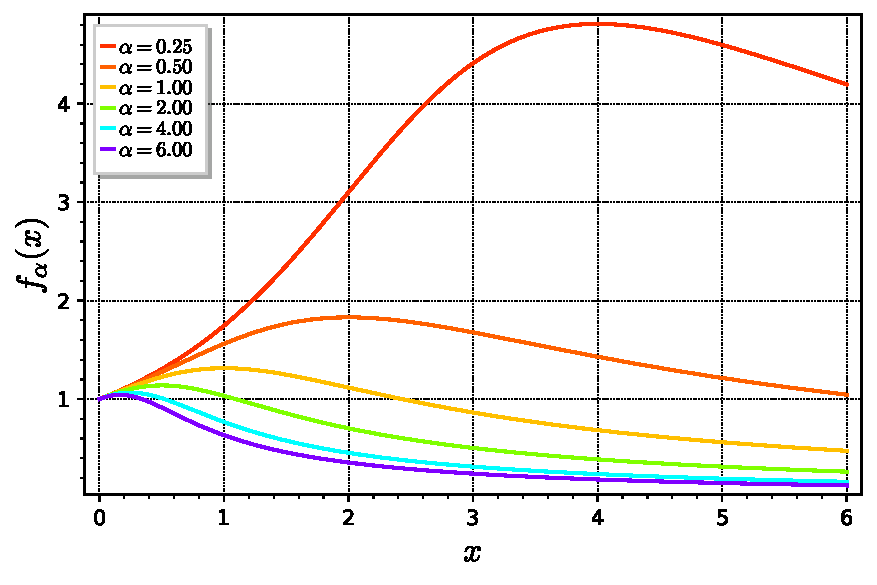
\includegraphics[width=0.6\textwidth]{vai_f_alpha_x.pdf}}
\caption[]{\label{f:vai:f_alpha_x} \footnotesize
Function $f_\alpha(x)$, defined by Eq.~(\ref{e:vai:sol_r_x_v0_small}),
for some selected values of $\alpha$. For each value of $\alpha$, the maximum
of $f_\alpha(x)$ is achieved for $x=1/\alpha$.
}
\end{figure}

It appears clearly on Eq.~(\ref{e:vai:eq_out_v0_small}) that
the homothety $H_\lambda:\ (t, r) \mapsto (\lambda t, \lambda r)$
transforms the geodesic $\Li_{(r_0,\th,\ph)}$ into the geodesic $\Li_{(\lambda r_0,\th,\ph)}$,
in agreement with the homothetic symmetry of the radiation region discussed
above.

Some outgoing radial null geodesics are depicted as solid green lines
in Fig.~\ref{f:vai:diag_S0}. In the radiation region, they obey
Eq.~(\ref{e:vai:eq_out_v0_small}).
Note that the homothetic symmetry appears clearly on the figure.
If a geodesic $\Li_{(r_0,\th,\ph)}$ has a turning point in terms of $r$ in the
radiation region, it must located at $x = 1/\alpha$, i.e. at $t/r = 1/\alpha - 1$,
or equivalently at
\be \label{e:vai:r_max_out}
  t = \left( \frac{v_0}{2m} - 1 \right) r .
\ee
The above equation defines a straight line through $(t,r) = (0,0)$,
whose intersection with the radiation region is depicted by a red segment
in Fig.~\ref{f:vai:diag_S0}.
\begin{remark}
The turning point value (\ref{e:vai:r_max_out}) can be obtained
directly by setting $\D r / \D t = 0$ in Eq.~(\ref{e:vai:ODE_outgoing_null})
and using the value (\ref{e:vai:S_linear}) for $M(v)$.
\end{remark}

In the Minkowski region, the outgoing radial null geodesics are straight line
segment inclined at $+45^\circ$ in Fig.~\ref{f:vai:diag_S0}, while
in the Schwarzschid region, they are curves obeying Eq.~(\ref{e:sch:outgoing_null_geod_EF})
(with the change of notation $\ti \leftrightarrow t$).


\subsection{Black hole formation}

In spherical symmetry, the inspection of the radial null geodesics gives us
a direct access to the black hole event horizon.
Let us determine the location of the latter for the homothetic
shell collapse considered above, since we have at disposal the exact solution
(\ref{e:vai:eq_out_v0_small}) for the outgoing radial null geodesics.



$t_{\rm hb}$ say\footnote{As in Chap.~\ref{s:lem}, the subscipt `hb' stands
for \emph{horizon birth}.}



\subsection{Curvature singularity}

The Kretschmann scalar\index{Kretschmann scalar!of Vaidya metric}
$K := R_{\mu\nu\rho\sigma} R^{\mu\nu\rho\sigma}$
(cf. Sec.~\ref{s:sch:singularities})
is computed in the notebook~\ref{s:sam:Vaidya}:
\be
    K = \frac{48 M(t + r)^2}{r^6} .
\ee
$K$ is identically zero in the Minkowski region ($M(r+t) = 0$), as it should!
It diverges at $r=0$ in the radiation and Schwarzschild regions, tracing the
existence of a curvature singularity there. Note that the curvature
singularity appears as soon as the radiation arrive at $r=0$, i.e. for
$t=0$ (cf. Fig.~\ref{f:vai:diag_S0}).

\begin{remark}
The Kretschmann scalar of Vaidya metric has the same structural form
as that of the Schwarzschild metric, compare Eq.~(\ref{e:sch:value_Kretschmann}),
while a priori $K$ could have
contained some term involving the derivative of $M(v)$. Indeed $M'(v)$
appears in some components of the Riemann tensor, since it is present in the
components of the Ricci tensor, as given by Eq.~(\ref{e:vai:Ricci_tensor}).
\end{remark}

\begin{remark}
Since the Ricci tensor of the Vaidya metric is not identically zero
[cf. Eq.~(\ref{e:vai:Ricci_tensor})], other curvature invariants that one might
have think of to track the curvature singularity are the Ricci scalar $R := g^{\mu\nu} R_{\mu\nu}$
and the Ricci ``squared'' $R_{\mu\nu} R^{\mu\nu}$. However, they are both identically zero
since $\w{k}$ is a null vector.
\end{remark}




\begin{figure}
\centerline{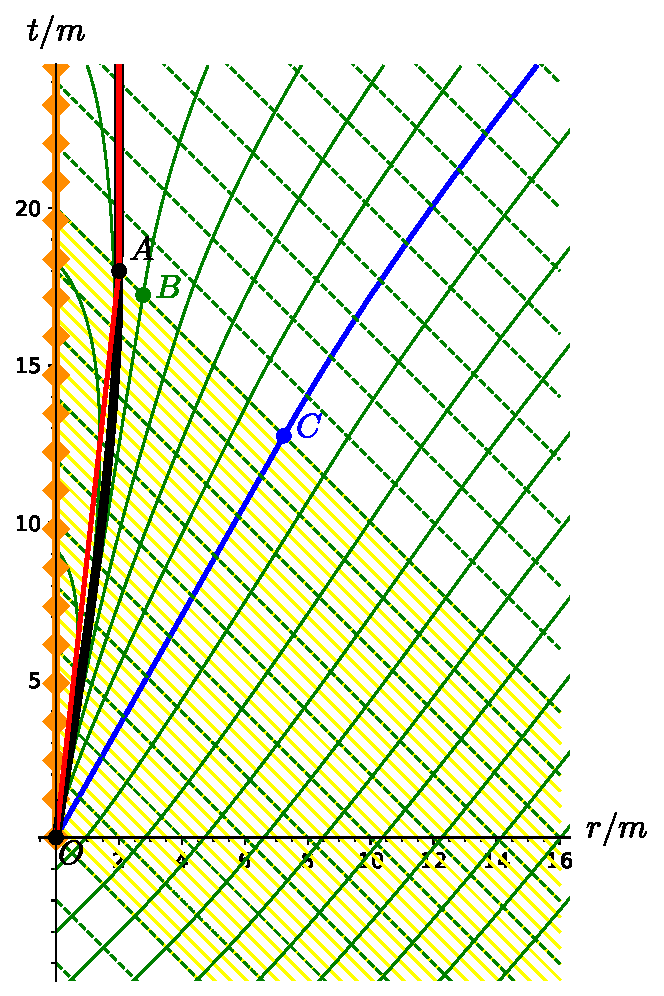
\includegraphics[width=0.6\textwidth]{vai_diag_naked_S0.pdf}}
\caption[]{\label{f:vai:diag_naked_S0} \footnotesize
Spacetime diagram of the Vaidya collapse based on the IEF coordinates $(t, r)$
and for the linear mass function $M(v)=m v/v_0$ with $v_0 = 20 m$.
The legend is the same as in Fig.~\ref{f:vai:diag_S0}, with in addition
the blue line marking the Cauchy horizon induced by the naked singularity
at $(t,r) = (0,0)$.
\textsl{[Figure generated by the notebook \ref{s:sam:Vaidya}]}
}
\end{figure}




%%%%%%%%%%%%%%%%%%%%%%%%%%%%%%%%%%%%%%%%%%%%%%%%%%%%%%%%%%%%%%%%%%%%%%%%%%%%%%%

\section{Trapping horizon}






%\section{Going further}

%\cite{Krish14}









